% !TEX root = ../intro-stellar-physics.tex

We saw in chapter~\ref{ch.basic-stellar-properties} that the equilibrium central temperature of a self-gravitating object---such as a star---with an ideal gas EOS depends \emph{solely} on the mass, radius, and composition of that star. For the Sun, this temperature is $\approx \val{15}{\Mega\K}$ and much higher than the surface effective temperature $T_{\!\mathrm{eff,\odot}} = \val{5780}{\K}$. The photons emitted from the Sun are coming from the cooler surface layers.

\newthought{Photons in a plasma, such as in the interior of the sun, transport energy.}  Were the sun transparent, these photons would immediately stream out, and the sun would release its stored energy in a fiery blast.  This doesn't happen: a photon can only travel a short distance before being scattered or absorbed. The net effect is that radiation generated in the core must travel a tortuous path, rather like a pinball, before reaching the surface and escaping.

\section{Interaction of radiation and matter}\label{s.interaction-radiation-matter}

How far does a photon---or any particle, for that matter---travel, on average, in the interior of the sun? Imagine a particle traveling with speed $v$.  Draw a cylinder, of length $\ell$ and cross-sectional area $\mathcal{A}$, around its future path, as shown in Fig.~\ref{f.MFP}. What the particle ``sees'' is that the cylinder is partly blocked by obstacles---other particles in its path. What is the probability of our particle making it through the cylinder unscathed?

\begin{marginfigure}
    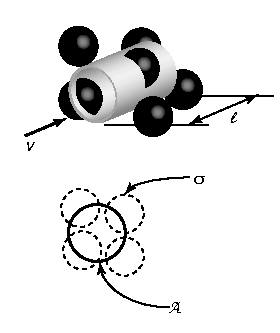
\includegraphics[width=\linewidth]{mean-free-path}
    \caption{\label{f.MFP} Schematic of a particle incident on a group of particles.}
\end{marginfigure}

The probability of the particle making it through is the ratio
\[
    \mathcal{P} = \frac{\textrm{total area covered by obstacles}}{\textrm{area of cylinder}}
\]
Denote the cross-sectional area of the other particles by $\sigma$.  If the density of obstacles is $n$, then the number of obstacles in the cylinder is $n\times(\mathcal{A}\ell)$, and therefore the fraction of the area blocked by the obstacles is
\begin{equation}
    \mathcal{P} = \frac{n\times(\mathcal{A}\ell)\times\sigma}{\mathcal{A}} = n\sigma\ell.
\label{e.prob-MFP}
\end{equation}
\marginnote{We are taking $\ell$ and $\mathcal{A}$ sufficiently small that we don't have to worry about particles overlapping.}
The particle will suffer a collision when $\mathcal{P}\to 1$, or when
\begin{equation}\label{e.MFP}
    \ell = \frac{1}{n\sigma}.
\end{equation}
We call $\ell$ the ``mean free path''.

\begin{exercisebox}[Mean free path for electron scattering]\label{ex.MFP}
    In the sun, free electrons scatter photons, and the cross-section is
    \[
    \sigma_{\mathrm{Th}} = \left(\frac{8\pi}{3}\right)\left(\frac{e^2}{m_e c^2}\right)^2 = \val{\sci{6.65}{-27}}{\meter^2}.
    \]
    What is the mean free path against this process for a photon at the average density of the solar interior?
\end{exercisebox}

\begin{exercisebox}[Mean free path of a hockey puck]\label{ex.MFP-2D}
    Suppose we have a flat surface on which pucks are sliding around, as shown in Fig.~\ref{f.MFP-2D} (Think of an air hockey table). The pucks bounce off the walls as they slide around.  Suppose there are $N$ pucks, each with a unit diameter, and the table is square with sides of length $L$.  Estimate the mean free path of a puck.
\end{exercisebox}

\begin{marginfigure}[-5\baselineskip]
    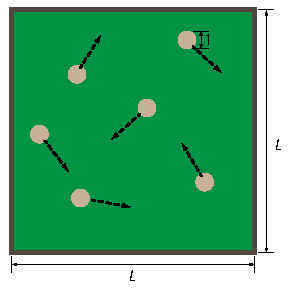
\includegraphics[width=\linewidth]{air-hockey-mfp}
    \caption[Mean free path of a hockey puck]{\label{f.MFP-2D}Schematic for Exercise~\ref{ex.MFP-2D}}
\end{marginfigure}

\newthought{Suppose we have a ray of light traversing some matter.} Over a small distance $\Delta s$, the probability of a photon being absorbed is $\mathcal{P} = n\sigma\Delta s$. Thus, out of every $N$ photons, $\Delta N = N \times\mathcal{P} = N\times n\sigma\Delta s$ are absorbed. Since the intensity $I_{\nu}$ is proportional to the number of photons, the change in intensity is just
\[ \Delta I_{\nu} = -n\sigma I_{\nu}\Delta s; \]
upon rearranging and taking the limit $\Delta s\to0$, we obtain an equation for the absorption of light,
\begin{equation}\label{e.absorption-microscopic}
\DD{I_{\nu}}{s} = -n\sigma I_{\nu}.
\end{equation}
Rather than work with the microscopic cross-section, it is convenient to define the \textbf{opacity},
\[
	\kapabs = \frac{n\sigma}{\rho},
\]
so that $\dif I_{\nu}/\dif s = -\rho\kapabs I_{\nu}$. The units of opacity are $\cm^{2}/\gram$. We use a subscript $\nu$ to indicate that the opacity is a function of frequency.

\begin{exercisebox}[Attenuation of light in an absorbing medium]
A ray of light crosses a slab of absorbent material. Calculate the intensity $I_{\nu}$ as a function of distance traveled. Your expression should be in terms of $\rho$ and $\kapabs$. How far does the ray go before its intensity has dropped to $1/e$ of its original value?
\end{exercisebox}

\newthought{In addition to absorbing photons, the matter can also spontaneously emit them.} Denote the power emitted per wavelength per volume per angle by $\rho j_{\nu}$. After traveling a distance $\Delta s$, the ray has increased in intensity by $\rho j_{\nu}\Delta s$, or
\begin{equation}\label{e.emission-microscopic}
\DD{I_{\nu}}{s} = \rho j_{\nu}.
\end{equation}

\begin{exercisebox}[Combined absorption and emission]
Suppose a ray traverses matter that both absorbs (opacity $\kapabs$) and emits (emissivity $j_{\nu}$), so that
\[	\DD{I_{\nu}}{s} = \rho j_{\nu} - \rho\kapabs I_{\nu}. \]
Solve for $I_{\nu}(s)$, and show that as $s\to\infty$, $I_{\nu}\to j_{\nu}/\kapabs$.
\end{exercisebox}

\newthought{Finally, the matter can also scatter light.} This removes light, similar to absorption, but then the light is put back into a different ray. If the intensity in our ray is greater than the angle-average $J_{\nu}$, scattering will cause a net reduction in intensity as more photons are scattered out of the ray than are scattered into it. Conversely, if $I_{\nu} < J_{\nu}$, then more photons will be scattered into the ray than out of it. Thus, the effect of scattering can be described via
\begin{equation}\label{e.scattering-microscopic}
\DD{I_{\nu}}{s} = -\rho\kapscat \left(I_{\nu} - J_{\nu}\right).
\end{equation}
Putting everything together gives us our full expression for how the intensity changes,
\begin{equation}\label{e.transfer-equation}
\DD{I_{\nu}}{s} = -\rho\left(\kapabs + \kapscat\right) I_{\nu} + \rho j_{\nu} + \rho\kapscat J_{\nu}.
\end{equation}
This is a complicated \textbf{integro-differential} equation: it contains both the derivative $\dif I_{\nu}/\dif s$ of the intensity as well as its integral $J_{\nu} = (4\pi)^{-1}\int I_{\nu}\,\dif\Omega$.

In general, eq.~(\ref{e.transfer-equation}) must be solved numerically; but conditions in the deep interior of the star and near the surface allow us to make simplifying approximations and to obtain a solution that gives some insight into the physics. First, let's clean up the equation: divide through by $\rho(\kapabs + \kapscat)$,
\[
	\frac{1}{\rho(\kapabs+\kapscat)}\dd{I_{\nu}}{s} = -I_{\nu} + \left[\frac{j_{\nu} + \kapscat J_{\nu}}{\kapabs + \kapscat}\right].
\]
Next, define a new quantity, the \textbf{optical depth} $\tau_{\nu}$ via the equation
\[
	\dd{\tau_{\nu}}{s} = \rho(\kapabs+\kapscat),
\]
which allows us to change variables, $\dif I_{\nu}/\dif s = (\dif I_{\nu}/\dif\tau_{\nu})\cdot(\dif\tau_{\nu}/\dif s)$; and finally define the \textbf{source function} $S_{\nu}$ as the term in $\left[\cdot\right]$. Doing all that gives us the simpler-looking equation,
\[
	\DD{I_{\nu}}{\tau_{\nu}} = -I_{\nu} + S_{\nu}.
\]
This doesn't advance us any closer to the solution, but notice! The optical depth has a simple meaning:
\[
	\tau_{\nu} = \int_{0}^{s} \rho(\kapabs+\kapscat)\,\dif s = \int_{0}^{s} n\sigma_{\nu}\,\dif s = \int_{0}^{s} \frac{\dif s}{\lambda}.
\]
That is, the optical depth measured the distance traveled, in units of mean free path. Said differently, if you have traveled one optical depth, then you have gone one mean free path.

Thus, if your object has $\tau_{\nu}\ll 1$, then photons are hardly affected by the medium and the object is nearly transparent; if, on the other hand, $\tau_{\nu} \gg 1$, then photons cannot go through the object: it is opaque.

\begin{exercisebox}[Optical depth of the solar center]
For the electron scattering cross-section (Exercise~\ref{ex.MFP}), estimate the optical depth between the solar center and the solar photosphere.
\end{exercisebox}

\newthought{Suppose we are in a cavity in which the radiation and matter are in a steady-state}. 
The matter is not gaining or losing energy to the radiation. This requires balancing
\[ \left(\textrm{energy emitted per unit volume}\right) = \rho\int j_{\nu}\,\dif\nu\,\dif\Omega\] 
with
\[ \left(\textrm{energy absorbed per unit volume}\right) = \rho\int \kapabs I_{\nu}\,\dif\nu\,\dif\Omega,\]
or
\begin{equation}\label{e.rad-equil}
\int_{0}^{\infty}\! \left(j_{\nu} - \kapabs J_{\nu}\right)\,\dif\nu = 0.
\end{equation}
We don't include scattering because it doesn't transfer energy between the radiation and the gas.

If, in addition, the matter and radiation are in thermal equilibrium, so that $J_{\nu} = B_{\nu}$, then
\begin{equation}\label{e.detailed-balance}
\frac{j_{\nu}}{\kapabs} = B_{\nu}(T).
\end{equation}
Notice that $j_{\nu}$ and $\kapabs$ are properties of the matter, and do not depend on the state of the radiation field. Hence, equation~(\ref{e.detailed-balance}) must hold whenever the matter is in equilibrium, \emph{regardless of the state of the radiation field}.

\section{Diffusion}\label{s.diffusion}

In the presence of scattering or absorption, the photons crossing the face can travel one mean free path $\ell$. Imagine a small cube with sides of length $\ell$ and filled with photons. The total radiant energy in the cube is $\Delta E$. In a time $\Delta t = \ell/c$, all of the energy will leave this cube. The total luminosity is $\Delta E/\Delta t = c\Delta E/\ell$. If everything is isotropic, then the flux out of any one face is $1/6$ of the luminosity, divided by the area of that face:
\[
	F = \frac{1}{6\ell^{2}}\frac{c\Delta E}{\ell} = \frac{1}{6}c U,
\]
where $U = E/\ell^{3}$ is the radiative energy density. 

\begin{marginfigure}
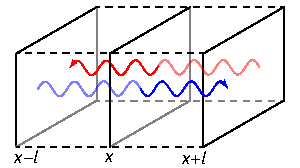
\includegraphics[width=\linewidth]{diffusive-flux}
\caption{\label{f.diffusive-flux} Illustration of net flux crossing a face between regions with slightly different energy densities.}
\end{marginfigure}
Now place two of these cubes against one another, with their common face located at position $x$. The energy density of the two cubes need not be the same; the energy density of the left cube is $U(x-\ell)$ and of the right cube is $U(x+\ell)$ (see Fig.~\ref{f.diffusive-flux}). The net flux traveling in the $x$-direction through the common face is then
\[
	F = {\color{blue}\frac{1}{6} c U(x-\ell)} - {\color{red}\frac{1}{6} c U(x+\ell)} \approx -\frac{1}{3}c\ell \DDx{U}.
\]
This is an expression for a \textbf{diffusive flux}. Although we gave a heuristic explanation, the formula is in general true:
\begin{eqnarray}
\nonumber
(\textrm{flux of something}) &=& -\frac{1}{3}\times(\textrm{speed of carriers})\times(\textrm{MFP of carriers})\\
&&\times \grad(\textrm{density of something})
\label{e.diffusive-flux}
\end{eqnarray}
For radiation, the ``something'' is ``radiative energy'' and the carriers are photons.

\newthought{Relate to random walk}


